\subsection{Solstrålning genom fönster}

%Skapat med sunfigurestest
I figur \ref{fig:sun0415and1231} ses de relevanta vinklar som bildas av solens position den 15 april 2011 (heldragna linjer), samt den 31 december 2011 (streckade linjer), beräknat med funktionen sunposition i appendix \ref{app:sunposition}. Den röda linjen visar solens höjd över horisonten medan den gröna indikerar solens azimuthala vinkel, det vill säga vinkel i sidled från en referenspunkt, här tagen till ostlig riktning och positivt medsols. Slutligen representerar den blå linjen i figuren solens vinkel relativt en vertikal ytas normal (då denna pekar i horisontell sydlig riktning) och kan användas för att uppskatta effekten som solinstrålning bidrar till.

\begin{figure}[hpbt]
\centering
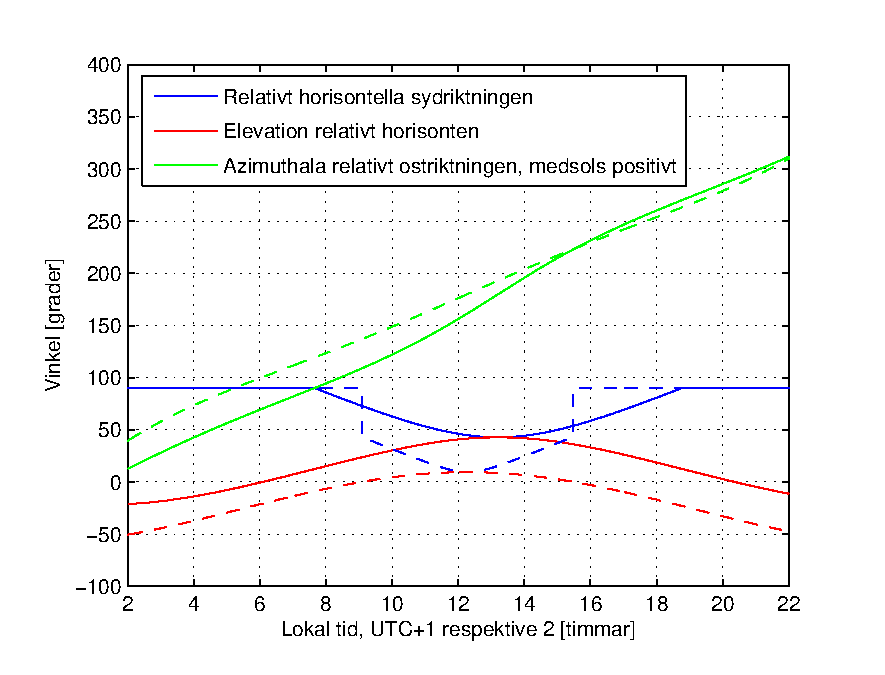
\includegraphics[scale=0.7]{images/sun0415and1231.eps}
\caption{\label{fig:sun0415and1231} Beräknade vinklar vid Walleriusgatan den 15 april 2011 (heldragna linjer, UTC+2) samt den 31 december samma år (streckade linjer, UTC+1).}
\end{figure}

Innan effekten beräknas måste dock ett exempel på solens intensitet över dagen skapas. Detta görs genom sambandet i avsnitt \ref{sec:sunthroughwindowsmethod}. Longitud och latitud för Walleriusgatan är ungefär 12 grader ost respektive 57,7 grader norr medan jordens medelradie är ungefär $\unit[6,731\cdot 10^{3}]{m}$ \cite{physicshandbook}. Den beräknade intensitet, som kan ses som de blå linjerna i figur \ref{fig:effekt0415and1231}, medför att effektflödet genom fönster kan beräknas.

\begin{figure}[hpbt]
\centering
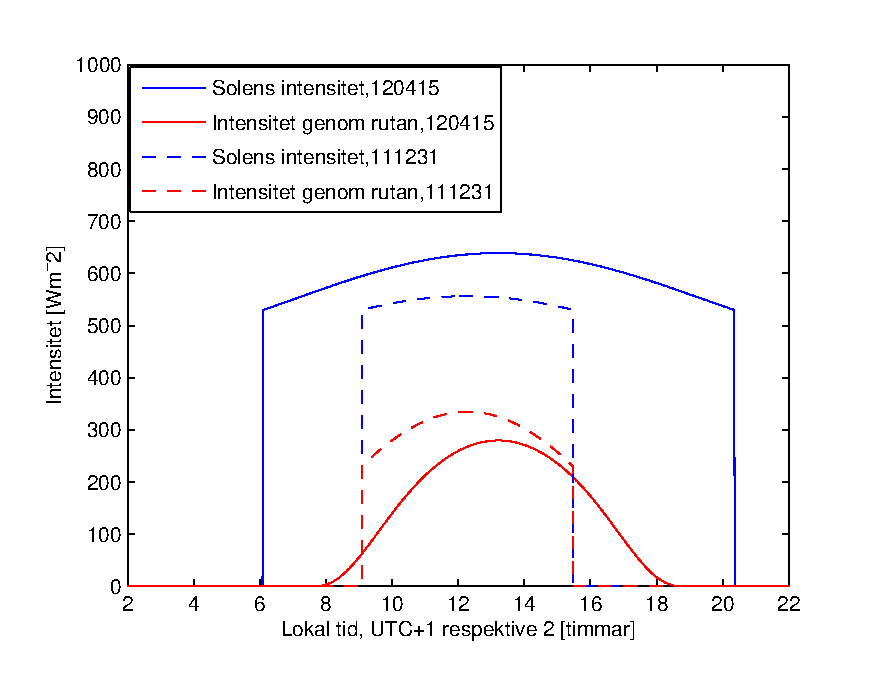
\includegraphics[scale=0.7]{images/effekt0415and1231.eps}
\caption{\label{fig:effekt0415and1231} Beräknad effekt genom ett fönster, vars normal pekar 38$^{\circ}$ öster om horisontella sydriktningen, den 15 april 2011 samt den 31 december samma år. Solens intensitet vid marknivå varierar under dagen enligt de blå kurvorna, resulterande i ett flöde genom fönstrena som följer de röda kurvorna. Notera att ingen hänsyn har tagits till skuggor eller persienner och dylikt.}
\end{figure}

Konstanterna q och p i ekvationen för g-värdet, \ref{eq:radiationwindowstheory:gvalue}, sätts till 4 respektive 3, ty fönstren i den avsedda byggnaden är av typ treglas utan ytbeläggningar. g-värdet för normal solstrålning, $g_0$,fås från \cite{ASHRAE09} till 0,61. Sydväggens normal pekar åt sydost, med vinkeln 38$^{\circ}$ mot horisontella sydriktningen. Dessa värden på konstanterna ger ett resultat, som kan ses i figur \ref{fig:effekt0415and1231}, för den 15 april 2011 och den 31 december samma år, indikerat med röda heldragna respektive streckade linjer.
